\section{Serveriosa}
Serveriosa arhitektuur on kihiline -- andmete töötlus alates andmebaasist küsimisest kuni kasutajale saatmiseni toimub neljas kihis:
\begin{itemize}
    \item andmebaasi ja domeeni kiht,
    \item andmete ligipääsu kiht,
    \item äriloogika kiht,
    \item andmete representeerimise kiht.
\end{itemize}
Kihtide eesmärk on selgelt eristada andmete töötlust loogika ja otstarve järgi. Andmete representeerimise kiht tegeleb andmete 
kasutajaliidesele saatmise ja kasutajaliideselt vastuvõtmisega ning ei pea mitte midagi teadma sellest, mis toimub andmetega hiljem --
see on äriloogika kihi töö. Analoogselt ka andmete ligipääsu kihis teostatakse ainult andmete küsimist ja salvestamist andmebaasile
(antud töö raames -- raamistiku kaudu), välistades igasugused infosüsteemi äriloogikaga seotud tegevused. Kihid on näidatu pildil

\begin{figure}[ht]
    \centering
    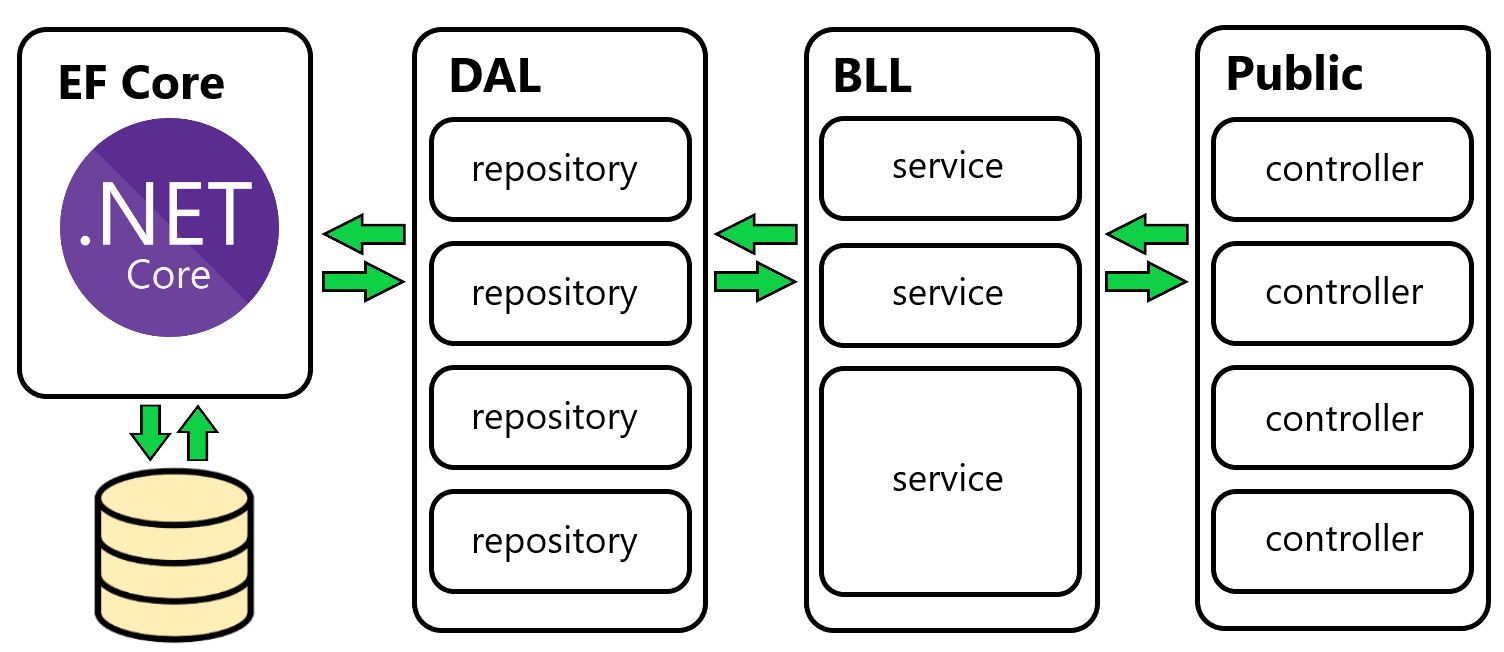
\includegraphics[width=1\textwidth]{figures/development/backend_structure.png}
    \caption[Serveriosa kihtide skemaatiline joonis]{\textit{Serveriosa kihtide skemaatiline joonis}}
    \label{fig:development_backend_layers}
\end{figure}
 

\textbf{Domain} (andmebaasi) kihis realiseeritakse projekteeritud andmebaasi mudel vastavate klassidena (näiteks \textit{Domain.App.Material},
\textit{Domain.App.Material-Category}, \textit{Domain.App.Material-Property} jne). Igas klassis määratakse vajalikud omadused ja
olemite vahelised seosed. Domain kiht moodustab andmebaasi konteksti (DbContext), mis on \textit{Entity Framework Core} raamistiku klass,
mille kaudu raamistik suhtleb andmebaasiga. Raamistiku kaudu luuakse andmebaasi genereerimise ja uuendamise skripte - migratsioone
(\textit{migration}). Kui üks olemite klassidest oli muudetud, siis võrdleb raamistik uue oleku eelmisega ning genereerib uue skripti.


\textbf{DAL} andmete ligipääsu kihis teostatakse tööd andmebaasi konstektsti objektiga (DbContext):  andmeid küsitakse Entity Framework Core-ist ja 
vastavalt ka salvestatakse \textit{DbContext}-isse. Kiht on jagatud üksusteks -- reposiooriumideks (\textit{Repository}), mis on 
baasimplementatsioonis kujutavad ennast klassikalist CRUD-tüüpi repositooriumi. Samuti repositooriumis 
teostatakse andmetele ligipääsu kontrolli kasutaja ID alusel -
nt meetod \textit{GetAllAsync(Guid uid, bool includePublic = false, String Include what, String)} küsib andmebaasist kõik olemid, 
mis kuuluvad kasutajale ID-ga \textit{uid} ning valikuliselt lisatakse ka olemeid, mis on ette nähtud ühiskasutuseks. 
Repositooriumiteks jagamist teostatakse andmemudeli ülesehituse alusel -- iga olemi jaoks on eraldi repositoorium. Selleks, et
äriloogika kihis erinevates teenustes oleks repositooriumite kasutamine paindlik, moodustatakse kõikidest repositooriumitest üks
objekt (\textit{UOW - Unit Of Work}), mille kaudu on võimalik juurde pääseda igale repositooriumile.

Kui rakendus vajab mõne olemi puhul keerulisemat repositooriumi loogikat, siis baasfunktsionaalsus saab olla üle kirjutatud
või laiendatud. Näiteks, materjalide (\textit{Domain.App.Material}) puhul on otstarbekam kohe agregeerida andmeid, 
mis puudutavad materjalide omadusi ((\textit{Domain.App.MaterialProperty}) ja (\textit{Domain.App.Property})), siis
äriloogika kihis ei pea tegema lisapäringuid, et teostada vajalikke arvutusi ja tegevusi.


\textbf{BLL} äriloogika kihis toimub kogu põhiline töö, mis on seotud vahetult rakenduse funktsionaalsust puudutava loogikaga.
Äriloogika kihi üksuseks on teenus (\textit{Service}). Teenuste moodustamise loogika suuresti vastab \textbf{DAL} kihi jagamise loogikale,
et võimalikult isoleerida erinevad teenused omavahelt. On ka teenused, mille eesmärk on erinevatest repositooriumitest andmete agregeerimine --
näiteks, arvutuste teenus (\textit{CalculationService}), mille otstarve on arvutusteks vajalike andmete komplekteerimine kasutajaliidesele
saatmiseks, kasutajaliideselt tulnud arvutuse päringu töötlemine, arvutuste teostamine ja arvutuse tulemuste tagastamine.
\textit{CalculationService} on äriloogika kihi kõike mahukam teenus. Kuna kalkulaatori tööks vajalike andmete maht on suur (materjalide
andmed, konstruktsioonide tüüpidega seotud andmed, sise- ja välistingimuste andmed), ei ole otstarbekas
neid kasutajaliidese poolelt küsida eraldi päringutega. Teenuses pannakse kokku andmete komplekt (\textit{dataset}), mida saadetakse
kasutajaliidesele ühe päringuga.





